\documentclass[12pt]{article}                                                                                                           
\usepackage[utf8]{inputenc}                                                                                                             
\usepackage[T1]{fontenc}                                                                                                                
\usepackage{amsmath, amssymb}                                                                                                           
\usepackage{geometry}                                                                                                                   
\usepackage{xcolor}                                                                                                                     
\usepackage{lipsum}                                                                                                                     
\usepackage{titlesec}                                                                                                                   
\usepackage{fancyhdr}                                                                                                                   
\usepackage{tcolorbox}                                                                                                                  
\usepackage{graphicx}                                                                                                                   
\usepackage{float} % For precise figure placement                                                                                       
\usepackage{tikz}                                                                                                                       
\usetikzlibrary{arrows.meta, decorations.markings}                                                                                      
\usepackage{geometry}
\usepackage{pgfplots}
\geometry{a4paper, margin=1in}                                           



\geometry{a4paper, margin=2.5cm}                                                                                                        
\pagestyle{fancy}                                                                                                                       
\fancyhf{}                                                                                                                              
\rhead{Problem Set II}                                                                                                                   
\lhead{Electricity I}                                                                                                                     
\cfoot{\thepage}                                                                                                                        
                                                                                                                                        
% Fancy titles                                                                                                                          
\titleformat{\section}{\normalfont\Large\bfseries}{Exercise \thesection:}{1em}{}                                                        
\titleformat{\subsection}{\normalfont\bfseries}{Correction:}{1em}{}                                                                     
                                                                                                                                        
% Custom box for correction                                                                                                             
\tcbuselibrary{listingsutf8}                                                                                                            
\newtcolorbox{correctionbox}{                                                                                                           
  colback=gray!5,                                                                                                                       
  colframe=black,                                                                                                                       
  fonttitle=\bfseries,                                                                                                                  
  title=Correction,                                                                                                                     
  breakable,                                                                                                                            
  before skip=10pt,                                                                                                                     
  after skip=10pt                                                                                                                       
}                                                                                                                                       
                                                                                                                                        
\begin{document}

% Cover info                                                                                                                            
\begin{center}
	\Large\textbf{UNIVERSITY IBN TOFAIL} \\[1em]
	\large\textit{Electricity I} \\[2em]
	\large\textit{Problem Set II} \\[0.5em]
\end{center}

\vspace{1cm}

% ----------- EXERCISE 1 -------------                                                                                                  
\section{}
Consider a sphere of radius $ R $ and center $ O $, uniformly charged with a positive volumetric charge density $ \rho $. A point $ M $ in space is identified by the distance $ OM = r $. Using Gauss's theorem, determine the electrostatic field $ \vec{E} $ created at this point $ M $.

\begin{correctionbox}
	\begin{align*}
		 & \textbf{Gauss's Law:}                                                                         \\
		 & \oint \vec{E} \cdot d\vec{S} = \frac{Q_{\text{enc}}}{\varepsilon_0},                          \\
		 & \text{where } Q_{\text{enc}} \text{ is the charge enclosed by the Gaussian surface.}
		\\
		 & \textbf{Case 1: Outside the Sphere ($ r > R $):}                                              \\
		 & \text{The total charge enclosed by the Gaussian surface is:}                                  \\
		 & Q_{\text{enc}} = \rho \cdot \text{Volume of sphere} = \rho \cdot \frac{4}{3} \pi R^3.         \\
		 & \text{Applying Gauss's law:}                                                                  \\
		 & E \cdot (4 \pi r^2) = \frac{\rho \cdot \frac{4}{3} \pi R^3}{\varepsilon_0}.                   \\
		 & \text{Solving for } E:                                                                        \\
		 & E = \frac{\rho R^3}{3 \varepsilon_0 r^2}.
		\\
		 & \textbf{Case 2: Inside the Sphere ($ r < R $):}                                               \\
		 & \text{The charge enclosed by the Gaussian surface is proportional to the volume of }          \\
		 & \text{the smaller sphere of radius $ r $:}                                                    \\
		 & Q_{\text{enc}} = \rho \cdot \text{Volume of smaller sphere} = \rho \cdot \frac{4}{3} \pi r^3. \\
		 & \text{Applying Gauss's law:}                                                                  \\
		 & E \cdot (4 \pi r^2) = \frac{\rho \cdot \frac{4}{3} \pi r^3}{\varepsilon_0}.                   \\
		 & \text{Solving for } E:                                                                        \\
	\end{align*}
\end{correctionbox}

\begin{correctionbox}
	\begin{align*}
		 & E = \frac{\rho r}{3 \varepsilon_0}. \\
		 & \textbf{Final Answer:}              \\
		 & E(r) =
		\begin{cases}
			\frac{\rho r}{3 \varepsilon_0},       & r \leq R, \\
			\frac{\rho R^3}{3 \varepsilon_0 r^2}, & r > R.
		\end{cases}
	\end{align*}
\end{correctionbox}

% ----------- EXERCISE 2 -------------                                                                                                  
\section{}
Consider an infinitely long cylinder of revolution along the $ OZ $-axis, with radius $ R $, carrying a uniform positive surface charge density $ \sigma $. Using Gauss's theorem, determine the electric field at any point in space.

\begin{correctionbox}
	\begin{align*}
		 & \textbf{Gauss's Law:}                                                                            \\
		 & \oint \vec{E} \cdot d\vec{S} = \frac{Q_{\text{enc}}}{\varepsilon_0},                             \\
		 & \text{where } Q_{\text{enc}} \text{ is the charge enclosed by the Gaussian surface.}
		\\
		 & \textbf{Symmetry Argument:}                                                                      \\
		 & \text{The electric field } \vec{E} \text{ is radial (perpendicular to the axis of the cylinder)} \\
		 & \text{and depends only on the radial distance } r \text{ from the axis.}
		\\
		 & \textbf{Case 1: Outside the Cylinder ($ r > R $):}                                               \\
		 & \text{The total charge enclosed by the Gaussian surface is:}                                     \\
		 & Q_{\text{enc}} = \sigma \cdot \text{Surface area of cylinder} = \sigma \cdot (2 \pi R L).        \\
		 & \text{Applying Gauss's law:}                                                                     \\
		 & E \cdot (2 \pi r L) = \frac{\sigma \cdot 2 \pi R L}{\varepsilon_0}.                              \\
		 & \text{Solving for } E:                                                                           \\
		 & E = \frac{\sigma R}{\varepsilon_0 r}.
		\\
		 & \textbf{Case 2: Inside the Cylinder ($ r < R $):}                                                \\
		 & \text{No charge is enclosed within the Gaussian surface because the charge resides only}         \\
		 & \text{on the surface of the cylinder. Thus:}                                                     \\
		 & E = 0.
		\\
		 & \textbf{Final Answer:}                                                                           \\
		 & E(r) =
		\begin{cases}
			0,                                & r \leq R, \\
			\frac{\sigma R}{\varepsilon_0 r}, & r > R.
		\end{cases}
	\end{align*}
\end{correctionbox}

% ----------- EXERCISE 3 -------------                                                                                                  
\section{}
Consider an infinite plane of negligible thickness, charged with a uniform positive surface charge density $ \sigma $. Using Gauss's theorem, determine the electric field created at a point on an axis perpendicular to the plane.

\begin{correctionbox}
	\begin{align*}
		 & \textbf{Gauss's Law:}                                                                                 \\
		 & \oint \vec{E} \cdot d\vec{S} = \frac{Q_{\text{enc}}}{\varepsilon_0},                                  \\
		 & \text{where } Q_{\text{enc}} \text{ is the charge enclosed by the Gaussian surface.}
		\\
		 & \textbf{Symmetry Argument:}                                                                           \\
		 & \text{The electric field } \vec{E} \text{ is perpendicular to the plane and has the same magnitude }  \\
		 & \text{on both sides of the plane.}                                                                    \\
		\\
		 & \textbf{Charge Enclosed:}                                                                             \\
		 & \text{For a cylindrical Gaussian surface passing through the plane, the charge enclosed is:}          \\
		 & Q_{\text{enc}} = \sigma \cdot \text{Area of one end of the cylinder} = \sigma A.
		\\
		 & \textbf{Flux Through the Gaussian Surface:}                                                           \\
		 & \text{The flux through the two flat ends of the cylinder is:}                                         \\
		 & \Phi = 2EA,
		\\
		 & \text{where } E \text{ is the magnitude of the electric field and } A \text{ is the area of one end.}
		\\
		 & \textbf{Applying Gauss's Law:}                                                                        \\
		 & 2EA = \frac{\sigma A}{\varepsilon_0}.
		\\
		 & \text{Solving for } E:                                                                                \\
		 & E = \frac{\sigma}{2 \varepsilon_0}.
		\\
		 & \textbf{Final Answer:}                                                                                \\
		 & \text{The electric field is constant and given by:}                                                   \\
		 & E = \frac{\sigma}{2 \varepsilon_0}.
	\end{align*}
\end{correctionbox}

% ----------- EXERCISE 4 -------------                                                                                                   
\section{}
In an orthonormal coordinate system $ (OXY) $, place three charges $ q_A > 0 $, $ q_B = q_A $, and $ q_C < 0 $ at points $ A(-d, 0) $, $ B(d, 0) $, and $ C(0, -d) $, respectively. Determine the electric potential $ V(y) $ created at a point $ M $ on the $ OY $-axis ($ \vec{OM} = y\hat{j} $).

\begin{correctionbox}
	\begin{align*}
		 & \textbf{Electric Potential Formula:}                                                                              \\
		 & \text{The electric potential due to a point charge } q \text{ at a distance } r \text{ is:}                       \\
		 & V = \frac{k q}{r}, \quad \text{where } k = \frac{1}{4 \pi \varepsilon_0}.
		\\
		 & \textbf{Distances from Charges to Point } M(0, y):                                                                \\
		 & \text{Distance from } A(-d, 0) \text{ to } M(0, y):                                                               \\
		 & r_A = \sqrt{d^2 + y^2}.
		\\
		 & \text{Distance from } B(d, 0) \text{ to } M(0, y):                                                                \\
		 & r_B = \sqrt{d^2 + y^2}.
		\\
		 & \text{Distance from } C(0, -d) \text{ to } M(0, y):                                                               \\
		 & r_C = |y + d|.
		\\
		 & \textbf{Potential Contributions:}                                                                                 \\
		 & \text{Potential due to } q_A:                                                                                     \\
		 & V_A = \frac{k q_A}{\sqrt{d^2 + y^2}}.
		\\
		 & \text{Potential due to } q_B:                                                                                     \\
		 & V_B = \frac{k q_B}{\sqrt{d^2 + y^2}}.
		\\
		 & \text{Potential due to } q_C:                                                                                     \\
		 & V_C = \frac{k q_C}{|y + d|}.
		\\
		 & \textbf{Total Potential:}                                                                                         \\
		 & \text{Adding the contributions:}                                                                                  \\
		 & V(y) = V_A + V_B + V_C = \frac{k q_A}{\sqrt{d^2 + y^2}} + \frac{k q_B}{\sqrt{d^2 + y^2}} + \frac{k q_C}{|y + d|}.
		\\
		 & \textbf{Final Answer:}                                                                                            \\
		 & \text{The electric potential is:}                                                                                 \\
		 & V(y) = \frac{k q_A}{\sqrt{d^2 + y^2}} + \frac{k q_B}{\sqrt{d^2 + y^2}} + \frac{k q_C}{|y + d|}.
	\end{align*}
\end{correctionbox}

% ----------- EXERCISE 5 -------------                                                                                                   
\section{}
Consider a disk of radius $ R $ and center $ O $, uniformly charged with a positive surface charge density $ \sigma $. Determine the electrostatic potential $ V(z) $ created by this system at a point $ M $ on its axis of revolution ($ OM = z $).

\begin{correctionbox}
	\begin{align*}
		 & \textbf{Charge Element Contribution:}                                                                   \\
		 & \text{Consider a small ring of radius } r \text{ and thickness } dr \text{ on the disk. The charge on } \\
		 & \text{this ring is:}                                                                                    \\
		 & dq = \sigma \cdot \text{Area of ring} = \sigma \cdot (2 \pi r dr).
		\\
		 & \textbf{Distance from Ring to Point } M(0, 0, z):                                                       \\
		 & \text{The distance from a point on the ring to } M \text{ is:}                                          \\
		 & r_M = \sqrt{r^2 + z^2}.
		\\
		 & \textbf{Potential Contribution from Ring:}                                                              \\
		 & \text{The potential due to the ring is:}                                                                \\
		 & dV = \frac{k dq}{r_M} = \frac{k \sigma (2 \pi r dr)}{\sqrt{r^2 + z^2}}.
		\\
		 & \textbf{Integrating Over the Disk:}                                                                     \\
		 & \text{Integrate } dV \text{ over the entire disk ($ r $ from $ 0 $ to $ R $):}                          \\
		 & V(z) = \int_0^R \frac{k \sigma (2 \pi r)}{\sqrt{r^2 + z^2}} dr.
		\\
		 & \textbf{Substitution:}                                                                                  \\
		 & \text{Let } u = r^2 + z^2, \text{ so } du = 2r dr. \text{ The limits change as follows:}                \\
		 & \text{When } r = 0, \, u = z^2,                                                                         \\
		 & \text{When } r = R, \, u = R^2 + z^2.
		\\
		 & \text{The integral becomes:}                                                                            \\
		 & V(z) = k \sigma \pi \int_{z^2}^{R^2 + z^2} \frac{du}{\sqrt{u}}.
		\\
		 & \textbf{Evaluate the Integral:}                                                                         \\
		 & \int \frac{du}{\sqrt{u}} = 2 \sqrt{u}.
		\\
		 & \text{Substituting back:}                                                                               \\
		 & V(z) = k \sigma \pi \left[ 2 \sqrt{R^2 + z^2} - 2 \sqrt{z^2} \right].
		\\
		 & \text{Simplify:}                                                                                        \\
		 & V(z) = 2 k \sigma \pi \left( \sqrt{R^2 + z^2} - |z| \right).
		\\
		 & \textbf{Final Answer:}                                                                                  \\
		 & \text{The potential is:}                                                                                \\
		 & V(z) = 2 k \sigma \pi \left( \sqrt{R^2 + z^2} - |z| \right).
	\end{align*}
\end{correctionbox}

% ----------- EXERCISE 6 -------------                                                                                                    
\section{}
A sphere of radius $ R $ is uniformly charged with a positive surface charge density $ \sigma $.
\begin{enumerate}
	\item Show that at any point outside the sphere, the electrostatic field is radial and identical to the field that would be created if the total charge of the sphere were concentrated at its center.
	\item Determine the value of the field inside the sphere and plot the graph $ E(r) $.
	\item Deduce the electrostatic potential at any point in space and plot its graph $ V(r) $.
\end{enumerate}

\begin{correctionbox}
	\begin{enumerate}
		\item Electric Field Outside the Sphere ($ r > R $),
		      Using Gauss's theorem, we calculate the electric field outside the sphere.
		      \begin{align*}
			       & \textbf{Gauss's Law:}                                                                        \\
			       & \oint \vec{E} \cdot d\vec{S} = \frac{Q_{\text{enc}}}{\varepsilon_0},                         \\
			       & \text{where } Q_{\text{enc}} \text{ is the total charge enclosed by the Gaussian surface.}
			      \\
			       & \textbf{Total Charge on the Sphere:}                                                         \\
			       & Q = \sigma \cdot \text{Surface area of sphere} = \sigma \cdot 4 \pi R^2.
			      \\
			       & \textbf{Electric Field Outside ($ r > R $):}                                                 \\
			       & \text{For a spherical Gaussian surface of radius } r > R, \text{ the enclosed charge is } Q. \\
			       & E \cdot (4 \pi r^2) = \frac{\sigma \cdot 4 \pi R^2}{\varepsilon_0}.
			      \\
			       & \text{Solving for } E:                                                                       \\
			       & E = \frac{\sigma R^2}{\varepsilon_0 r^2}.
			      \\
			       & \textbf{Conclusion:}                                                                         \\
			       & \text{The field outside the sphere is radial and identical to that created }                 \\
			       & \text{by a point charge}                                                                     \\
			       & Q \text{ at the center.}
		      \end{align*}
		\item Electric Field Inside the Sphere ($ r < R $),
		      Inside the sphere, the electric field is zero because the charge resides only on the surface.nside the sphere, the electric field is zero because the charge resides only on the surface.
		      \begin{align*}
			       & \textbf{Electric Field Inside ($ r < R $):}                          \\
			       & \text{No charge is enclosed within the Gaussian surface for } r < R. \\
			       & E = 0.
		      \end{align*}
		\item Electrostatic Potential $ V(r) $,
		      We now calculate the electrostatic potential in all space and plot $ V(r) $.
















	\end{enumerate}
\end{correctionbox}

\begin{correctionbox}
	\begin{align*}
		 & \textbf{Potential Outside the Sphere ($ r > R $):}                                \\
		 & V(r) = \frac{k Q}{r} = \frac{k (\sigma \cdot 4 \pi R^2)}{r}.
		\\
		 & \textbf{Potential Inside the Sphere ($ r < R $):}                                 \\
		 & \text{The potential inside the sphere is constant and equal to the potential at } \\
		 & \text{the surface:}                                                               \\
		 & V(r) = V(R) = \frac{k Q}{R} = \frac{k (\sigma \cdot 4 \pi R^2)}{R}.
		\\
		 & \textbf{Final Expression for Potential:}                                          \\
		 & V(r) =
		\begin{cases}
			\frac{k (\sigma \cdot 4 \pi R^2)}{R}, & r \leq R, \\
			\frac{k (\sigma \cdot 4 \pi R^2)}{r}, & r > R.
		\end{cases}
	\end{align*}
	\subsection*{Graphs of $ E(r) $ and $ V(r) $}
	We now plot $ E(r) $ and $ V(r) $ using \texttt{pgfplots}.

	\begin{center}
		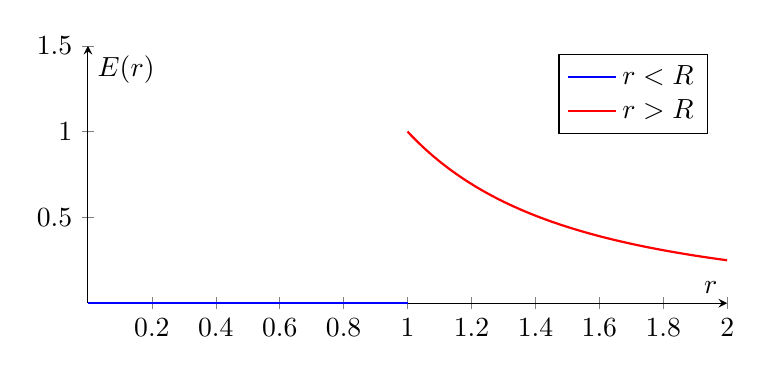
\begin{tikzpicture}
			\begin{axis}[
					xlabel={$ r $},
					ylabel={$ E(r) $},
					axis lines=middle,
					xmin=0, xmax=2,
					ymin=0, ymax=1.5,
					domain=0:2,
					samples=100,
					legend pos=north east,
					width=0.8\textwidth,
					height=0.4\textwidth,
				]
				% Electric Field Inside (r < R)                       
				\addplot[blue, thick] coordinates {(0,0) (1,0)};
				% Electric Field Outside (r > R)                      
				\addplot[red, thick, domain=1:2] {1/x^2};
				\legend{$ r < R $, $ r > R $};
			\end{axis}
		\end{tikzpicture}
	\end{center}

	\begin{center}
		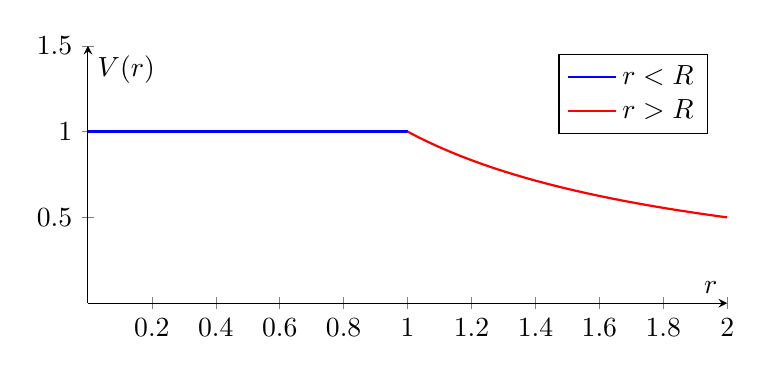
\begin{tikzpicture}
			\begin{axis}[
					xlabel={$ r $},
					ylabel={$ V(r) $},
					axis lines=middle,
					xmin=0, xmax=2,
					ymin=0, ymax=1.5,
					domain=0:2,
					samples=100,
					legend pos=north east,
					width=0.8\textwidth,
					height=0.4\textwidth,
				]
				% Potential Inside (r < R)                            
				\addplot[blue, thick] coordinates {(0,1) (1,1)};
				% Potential Outside (r > R)                           
				\addplot[red, thick, domain=1:2] {1/x};
				\legend{$ r < R $, $ r > R $};
			\end{axis}
		\end{tikzpicture}
	\end{center}
\end{correctionbox}

% ----------- the documents finishes here body :D -------------                                                                         
\end{document}
